%%%%%%%%%%%%%%%%%%%%%%%%%%%%%%%%%%%%%%%%%%%%%%%%%%%%%%%%%%%%%%%%%%%%%
\section{Motivating Example and Motivating questions} \label{sect:background}
%%%%%%%%%%%%%%%%%%%%%%%%%%%%%%%%%%%%%%%%%%%%%%%%%%%%%%%%%%%%%%%%%%%%%

This section motivates our work through an example and the motivation question to tackle the challenges.
%%%%%%%%%%%%%%%%%%%%%%%%%%%%%%%%%%%%%%%%%%%%%%
\subsection{Motivating Example} 
\label{sect:bg-courseman-eg}
%%%%%%%%%%%%%%%%%%%%%%%%%%%%%%%%%%%%%%%%%%%%%%

% ducmle: OLD
%\begin{figure*}[ht]
%	\begin{center}
%		\includegraphics[scale=0.28]{motivatingExample}
%	\end{center}
%	\caption{Simplified UML/OCL class and activity diagrams to specify a \courseman software variant that handles the enrolment management activity.} %
%	\label{fig:motivatingExample}
%\end{figure*} 
We adapt a compact and essential software domain from a previous work \cite{le_domain_2018}, named course management domain (\courseman) as our motivating example. We introduce here the basic \courseman requirements and use it to illustrate the background concepts. In the rest of the paper, we will use this example and, where necessary, some extensions of it to illustrate our proposed method.

\begin{figure}[th]
\begin{center}
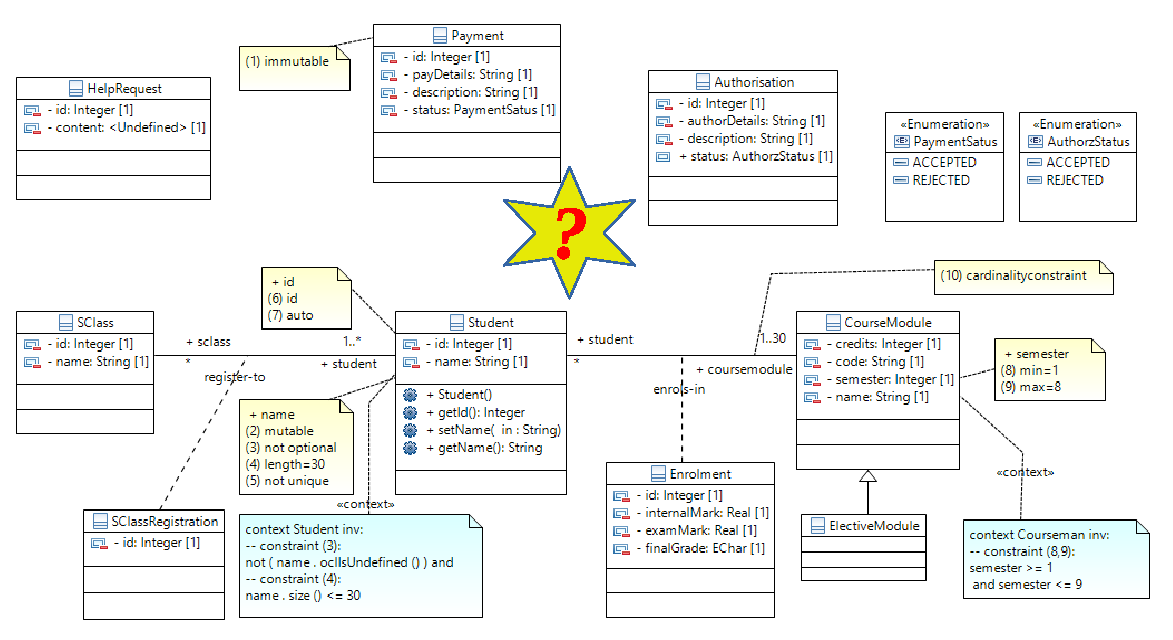
\includegraphics[scale=0.5]{motivating-example}
\end{center}
\caption{The essential domain model of \courseman.}
\label{fig:motivatingExample}
\end{figure}

The bottom part of Figure~\ref{fig:motivatingExample} shows four classes and two association classes of \Name{CourseMan}. Class \clazz{Student} represents students that register to study in an academic institution. Class \clazz{CourseModule} represents the course modules that are offered by the institution. Class \clazz{ElectiveModule} represents a specialized type of \clazz{CourseModule}. Class \clazz{SClass} represents the student class type for students to choose. Association class \clazz{\clazz{SClass}Registration} captures details about the many-many association between \clazz{Student} and \clazz{SClass}. Finally, association class \clazz{Enrolment} captures details about the many-many association between \clazz{Student} and \clazz{CourseModule}.
The top part of Figure~\ref{fig:motivatingExample} (the area containing a star-like shape labeled ``?'') shows three other classes that are intended to capture the design of an enrolment management activity. Suppose that we know some design details (the attributes shown in the figure) and the following description about these classes:
%
\begin{itemize}[noitemsep]
  \item \clazz{HelpRequest}: captures data about help information provided to students.
  \item \clazz{Payment}: captures data about payment for the intuition fee that a student needs to make.
  \item \clazz{Authorisation}: captures data about the decision made by an enrolment officer concerning whether or not to allow a student to undertake the registered course modules.
  % paragraph break
  %\\
\end{itemize}

We illustrate below how a number of common invariant constraints on \clazz{Student} and \clazz{CourseModule} are expressed in OCL \cite{omg_object_2014}. Other constraints are expressed using more complex OCL expressions and techniques, whose details (see \cite{le_domain_2018}) are beyond the scope of this paper.

%
\begin{lstrulex}
context (@\hterm{Student inv}@):
  -- constraint (@\hterm{(3)}@):
  not(name.oclIsUndefined()) and 
  -- constraint (@\hterm{(4)}@):
  name.size() <= 30

context (@\hterm{CourseModule inv}@):
  -- constraint (@\hterm{(8)}@):
  semester >= 1 and 
  -- constraint (@\hterm{(9)}@):
  semester <= 8
\end{lstrulex}

\begin{figure}[th]
	\begin{center}
		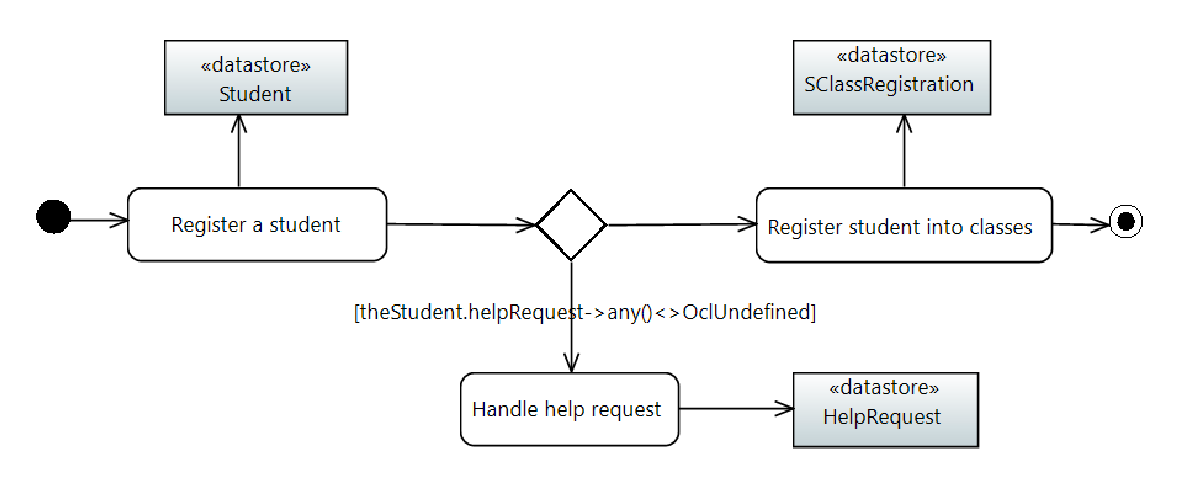
\includegraphics[scale=0.5]{motivating-example2}
	\end{center}
	\caption{Combining structural and behavioural \courseman models.}
	\label{fig:motivatingExample2}
\end{figure}

In practical applications, the class model is often combined with a behavioral model (\eg a UML activity diagram) to describe a unified view of the domain requirements. Throughout this paper, we will refer to this combined model as \textit{unified domain model}. For instance, the left-hand side of Figure~\ref{fig:motivatingExample2} illustrates the combination of a simple class diagram of \courseman (displayed at the bottom) and an activity diagram of the enrolment management function. This activity involves registering \clazz{Student}s, enrolling them into \clazz{CourseModule}s and registering them into \clazz{SClass}es. In addition, it would allow a \clazz{Student} to raise a \clazz{HelpRequest} during the enrolment process. 
The right-hand side of Figure~\ref{fig:motivatingExample2} depicts an unspecified unified domain model of the \courseman example. What this model entails and how this can be specified are the main questions that we seek to answer in this paper. We will state shortly a number of research questions relating to this model that we will specifically focus on investigating.

%Class \clazz{Student} represents the domain concept Student%
%\footnote{use \clazz{fixed~font} for model elements and normal font for concepts.}. %
%Class \clazz{Course} represents the Courses%
%\footnote{use class/concept name as countable noun to identify instances.} %
%that are offered to students. Class \clazz{SClass} represents types of classes (\eg morning, afternoon, and evening) that \clazz{Student}s
%can choose. 

%Class \clazz{EnrolmentMgmt} represents the enrolment management activity. This essentially involves registering \clazz{Student}s, enrolling them into \clazz{CourseModule}s and registering them into \clazz{SClass}es. In addition, it allows each \clazz{Student} to raise a \clazz{HelpRequest}. Throughout this paper, we will discuss different variants of this activity.
%The right-hand side of Fig.~\ref{fig:motivatingExample} depicts an activity diagram that captures behavioral aspects from the enrolment management activity.

% + (done) TODO: Duc
% - copy example from the 2018 Journal paper here
% - add the activity diagram EnrolmentMgmt (in this paper, we will extend this basic example to handle all the basic activity diagram patterns)

%%%%%%%%%%%%%%%%%%%%%%%%%%%%%%%%%%%%%%%%%%%%%%
%Move Backround to Section Background an related work
%
%%%%%%%%%%%%%%%%%%%%%%%%%%%%%%%%%%%%%%%%%%%%%%
\subsection{Motivating Questions}
%%%%%%%%%%%%%%%%%%%%%%%%%%%%%%%%%%%%%%%%%%%%%%

As illustrated by the motivating example, a unified domain model could be defined as a loose combination of (1)~a class diagram for a domain model, (2)~an activity diagram for domain behaviors, and (3)~OCL constraints attached to these specifications. This puts forward a need to incorporate domain behaviors into the domain model specified by the DCSL framework~\cite{le_domain_2018} for a unified model with the three features, as explained in Section~\ref{sect:bg-dcsl}, feasibility, productivity, and understandability. Note that the DCSL framework has been defined as an initial effort for the three key features by extending the class metamodel with new meta-concepts to express OCL-like constraints.
%in the form of annotations in the host language.
Specifically, to realize this approach, we need to tackle the following challenges:

\begin{itemize}
    \item How can we extend the DCSL framework with new constructs to represent domain behaviors that could be captured by UML activity diagrams?
    \item How can we define a mechanism to incorporate such domain behaviors into a DCSL-specified domain model? This requires us to define an integrated semantics of structural and behavioral aspects of a domain model.
\end{itemize}


